\chapter{Evaluation}
\label{sec:evaluation}
% Analyse on expressions instead of statements.
% Statements that contain a block should have not been split as this makes reconstruction very difficult.
Evaluating the success of my solution is difficult. My implemented solution only works for some examples, as only some features of the language are supported. It focus is on parallelising as much as possible, not necessarily on getting a faster program. \todo{Fact check this} Many research papers in the field compare their speedup to LLVM, but the rust compiler (like many languages) uses LLVM for the final stages of compilation. Optimisations from LLVM will be applied to both the sequential and parallel versions, and so my results may not be comparable to others.

Two sequential programs were parallelised: a simple example and a password cracker. The dependency tree and schedule are analysed to check the validity of the parallelising compiler. A collection of automatically generated sequential programs were also parallelised and their output was compared with the sequential version to check that the parallelisms have not semantically changed the program. The amount of concurrent threads was recorded, as well as performance of the parallel version is compared with the sequential version to see if the parallelisms have any affect.

\section{Sequential Programs Parallelised}
\subsection{Simple Example}
This simple example is intended as an easy example to understand how the parallelising compiler works. It consists of two independent variables, \texttt{a} and \texttt{b} which are printed together.

\begin{code}
    \inputcode{simple-example/main.rs}{}{}
    \caption{A simple example program}
\end{code}

\begin{figure}[H]
    \centering
    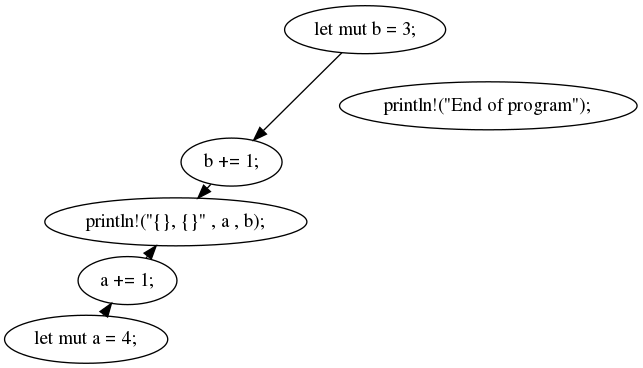
\includegraphics[width=0.6\textwidth]{img/simple-example/main-dependency-analysis.png}
    \caption{Dependency analysis graph of the simple example}
\end{figure}

The dependency analysis graph clearly shows \texttt{a} and \texttt{b} do not need to be inter-weaved. It also shows that the \texttt{println!(``End of program");} is completely independent of the other print statement. This may not be intended by the programmer, but there is nothing inside the \texttt{println!} macro which states that they must be called in order (there is no variable linking the two print statements). This could be fixed by forcing external functions to be executed in order, even if there is no variable linking them together. This would reduce the number of parallelisms detected, but it would make the programs more compatible. Because this dependency is not detected, I sorted the outputs of both sequential and parallel programs so that the order does not matter when comparing outputs.

\begin{figure}[H]
    \centering
    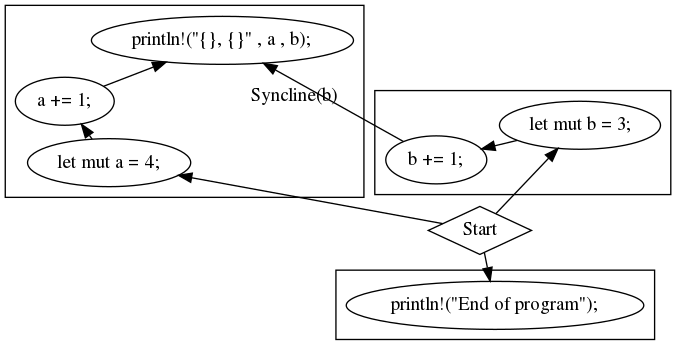
\includegraphics[width=0.6\textwidth]{img/simple-example/main-schedule.png}
    \caption{Schedule of the simple example}
\end{figure}

The scheduling algorithm split \texttt{a} and \texttt{b} into separate threads as well as the ``End of program" print statement. The print statement that prints \texttt{a} and \texttt{b} attached itself to the \texttt{a} thread. The \texttt{b} variable is sent along a syncline just before the print.

\subsection{Password Cracker}
The password cracker contains three functions: \texttt{loadDictionary()}, \texttt{hash()} and \texttt{main()}. The \texttt{loadDictionary()} is not analysed here as the parallelising compiler did not make any changes to this function. This program is on the limits of what my parallelising compiler can do in its current state. Some of the code is written specifically to get it to parallelise properly.

\subsubsection{Hash Function}
The hash function uses an external crate which implements SHA256. The word argument is iteratively hashed $1000$ times and then returned. Notice that \texttt{i} is set to decrease from $999$ to $0$ which does not have any impact on the loop. This has been added to disable the parallelising compiler from trying to parallelise this loop. Line $32$ has no dependencies and can be run in parallel. If it was computationally expensive to call \texttt{Sha256::new()} then it would make sense to run this statement of the loop in parallel. The rest of the statements depend on the previous iteration and so no speedup can be achieved here. Also note that \texttt{hash\_word} is borrowed on line $33$ which is not a \todo{is it borrowing, or the str type that breaks this?} fully supported feature of the parallelising compiler. For these reasons, I manually disabled the loop being parallelised in this case. If the performance analyse and borrowing features were implemented, the \texttt{.rev()} would not need to be added.

\begin{code}
    \inputcode{password-cracker/main.rs}{27}{37}
    \caption{Hash function of the password cracker program}
\end{code}

\begin{figure}[H]
    \centering
    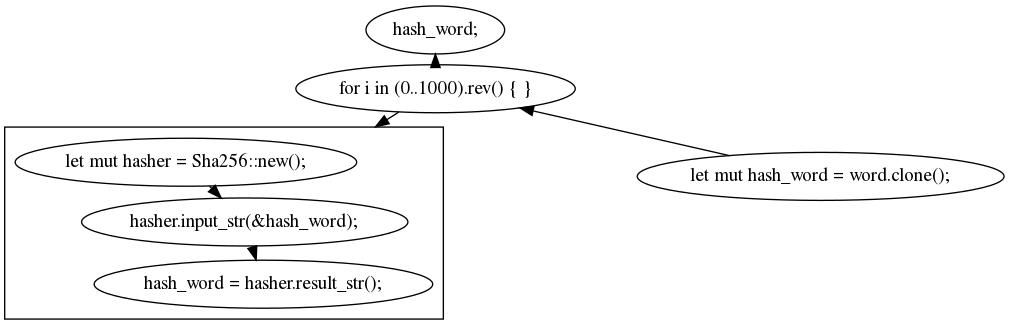
\includegraphics[width=\textwidth]{img/password-cracker/hash-dependency-analysis.png}
    \caption{Dependency analysis graph of the hash function from the password cracker program}
\end{figure}

The dependency graph shows how the inner block is linear for one iteration. The reason that the loop cannot be parallelised effectively is that \texttt{hash\_word} is modified each iteration.

\begin{figure}[H]
    \centering
    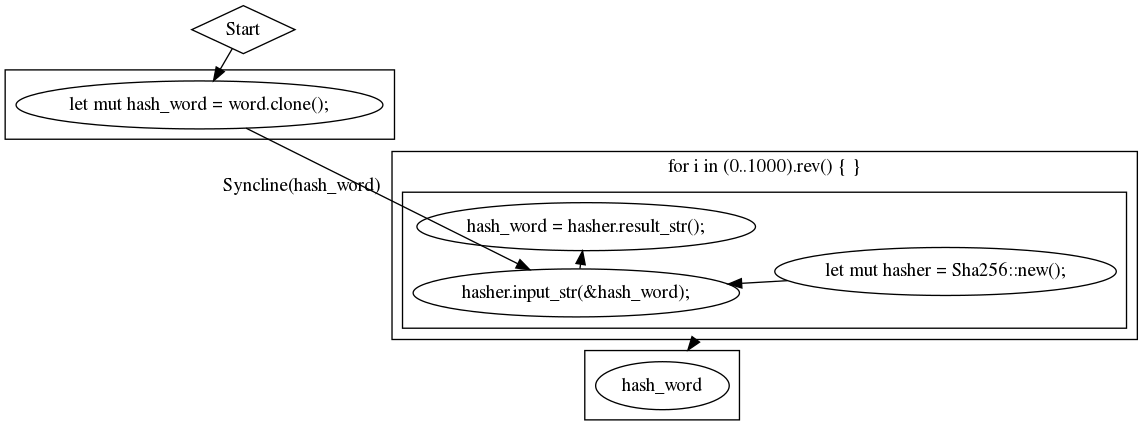
\includegraphics[width=0.6\textwidth]{img/password-cracker/hash-schedule.png}
    \caption{Schedule of the hash function from the password cracker program}
\end{figure}

The schedule shows how linear the iterative hash function is. The only thread separate thread that is spawned clones the word. The reason that the for loop is not inside the same thread is because the \texttt{hash\_word} dependency is inside the for loop. The condition on the for loop is independent and could be slow and so is parallelised. In reality, this will be much slower due to thread overhead.

\subsubsection{Main Method}
The main method loads the dictionary from a file into a list of strings. Each word in this list is hashed and compared with a password hash. Notice that the for loop is not interrupted when it finds the correct word, or even stored; it is just printed. A timing circuit is placed around the function to print how long it takes to find the password.
\begin{code}
    \inputcode{password-cracker/main.rs}{39}{57}
    \caption{Main method of the password cracker program}
\end{code}

\begin{figure}[H]
    \centering
    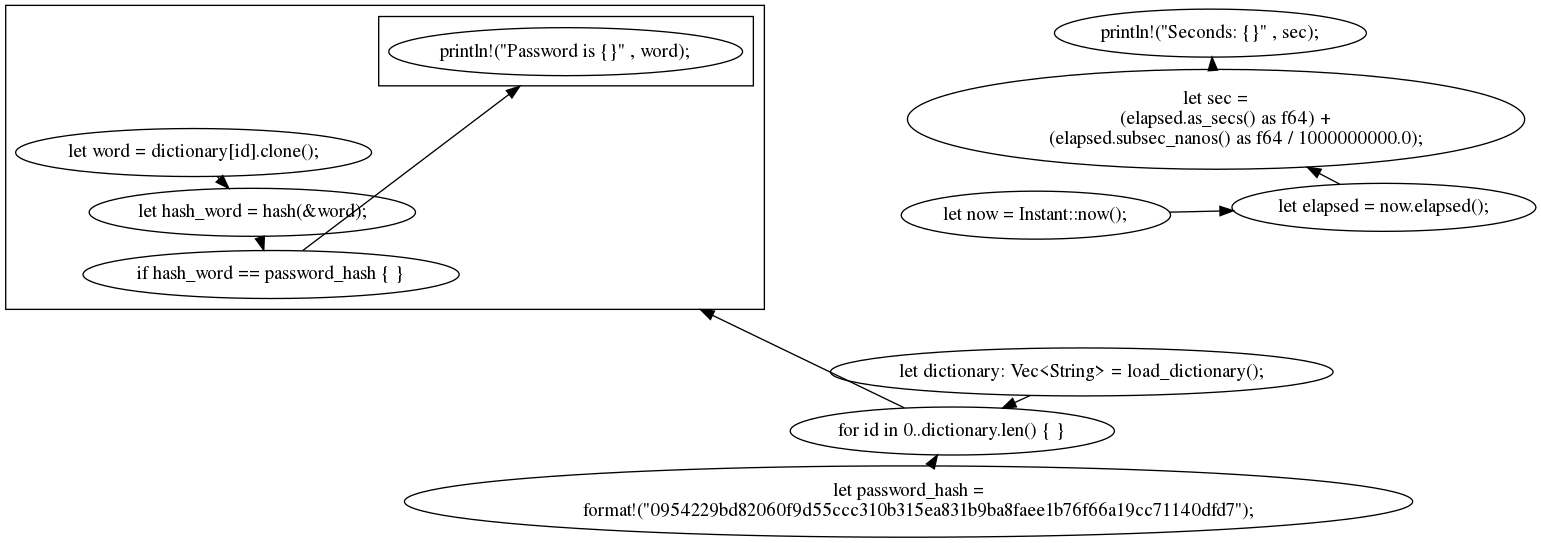
\includegraphics[width=\textwidth]{img/password-cracker/main-dependency-analysis.png}
    \caption{Dependency analysis graph of the main method from the password cracker program}
\end{figure}

As you can see from the dependency graph, the timing circuit is a completely independent program. This is probably not intended, and it is a similar problem to the \texttt{println!} problem. There is no real fix I can think of for this issue except hard coding the time crate to be dependent on everything (and everything dependent on it). I am not a fan of hard coding this, as there may be other functions in other crates which also have similar dependency requirements. I will just remove the timing circuit when comparing the outputs as the time will not be consistent between runs.

\begin{figure}[H]
    \centering
    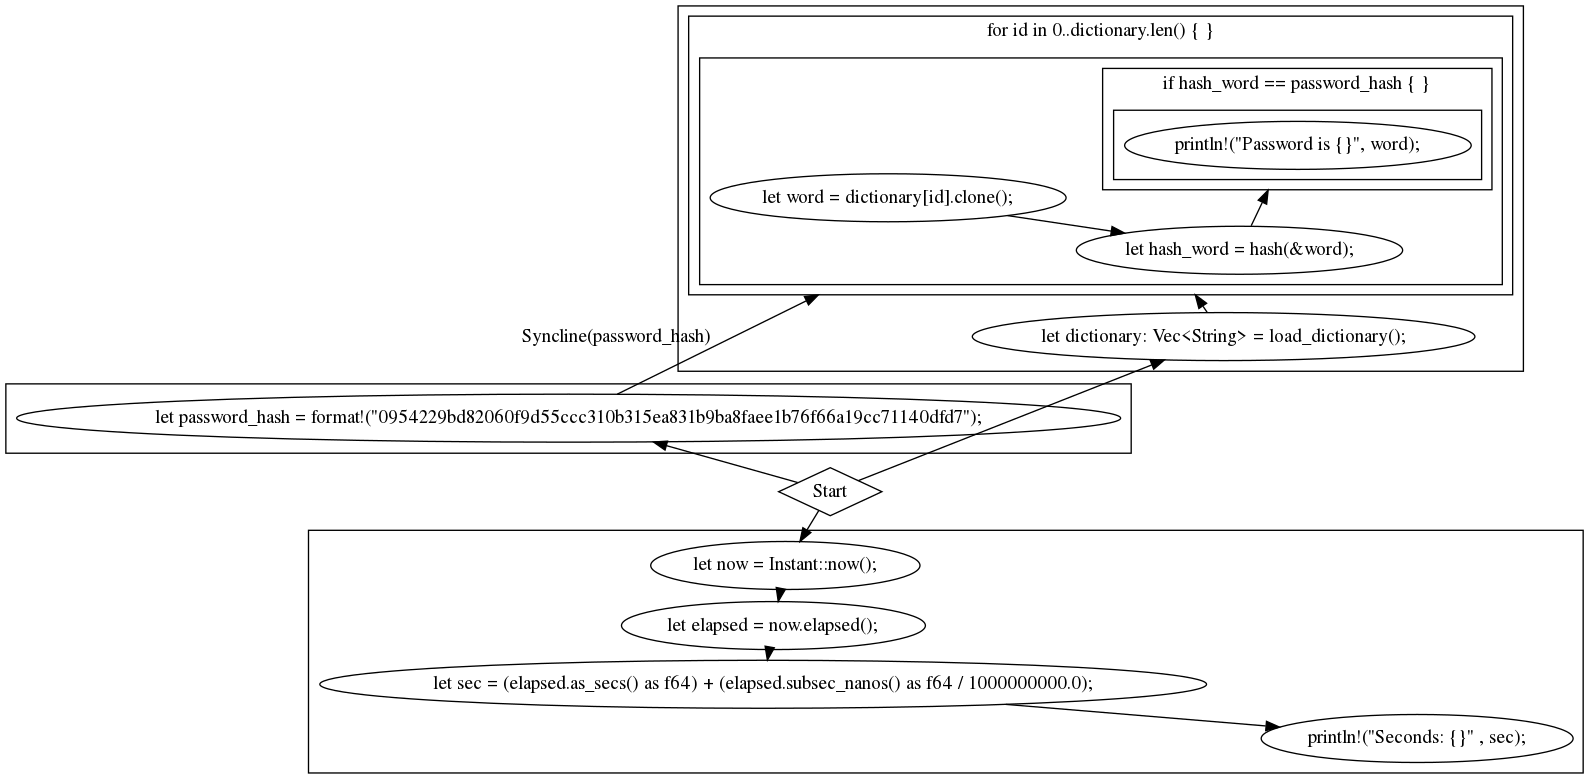
\includegraphics[width=\textwidth]{img/password-cracker/main-schedule.png}
    \caption{Schedule of the main method from the password cracker program}
\end{figure}

The schedule also shows that the timing circuit is separate. The \texttt{password\_hash} assignment is placed in its own thread, as the for loop condition is independent. The block inside the for loop does depend on this value, and so a syncline is setup. It is not clear from the schedule above, but the for loop is also parallelised. The schedule below shows the synclines between each iteration of the for loop.

\begin{figure}[H]
    \centering
    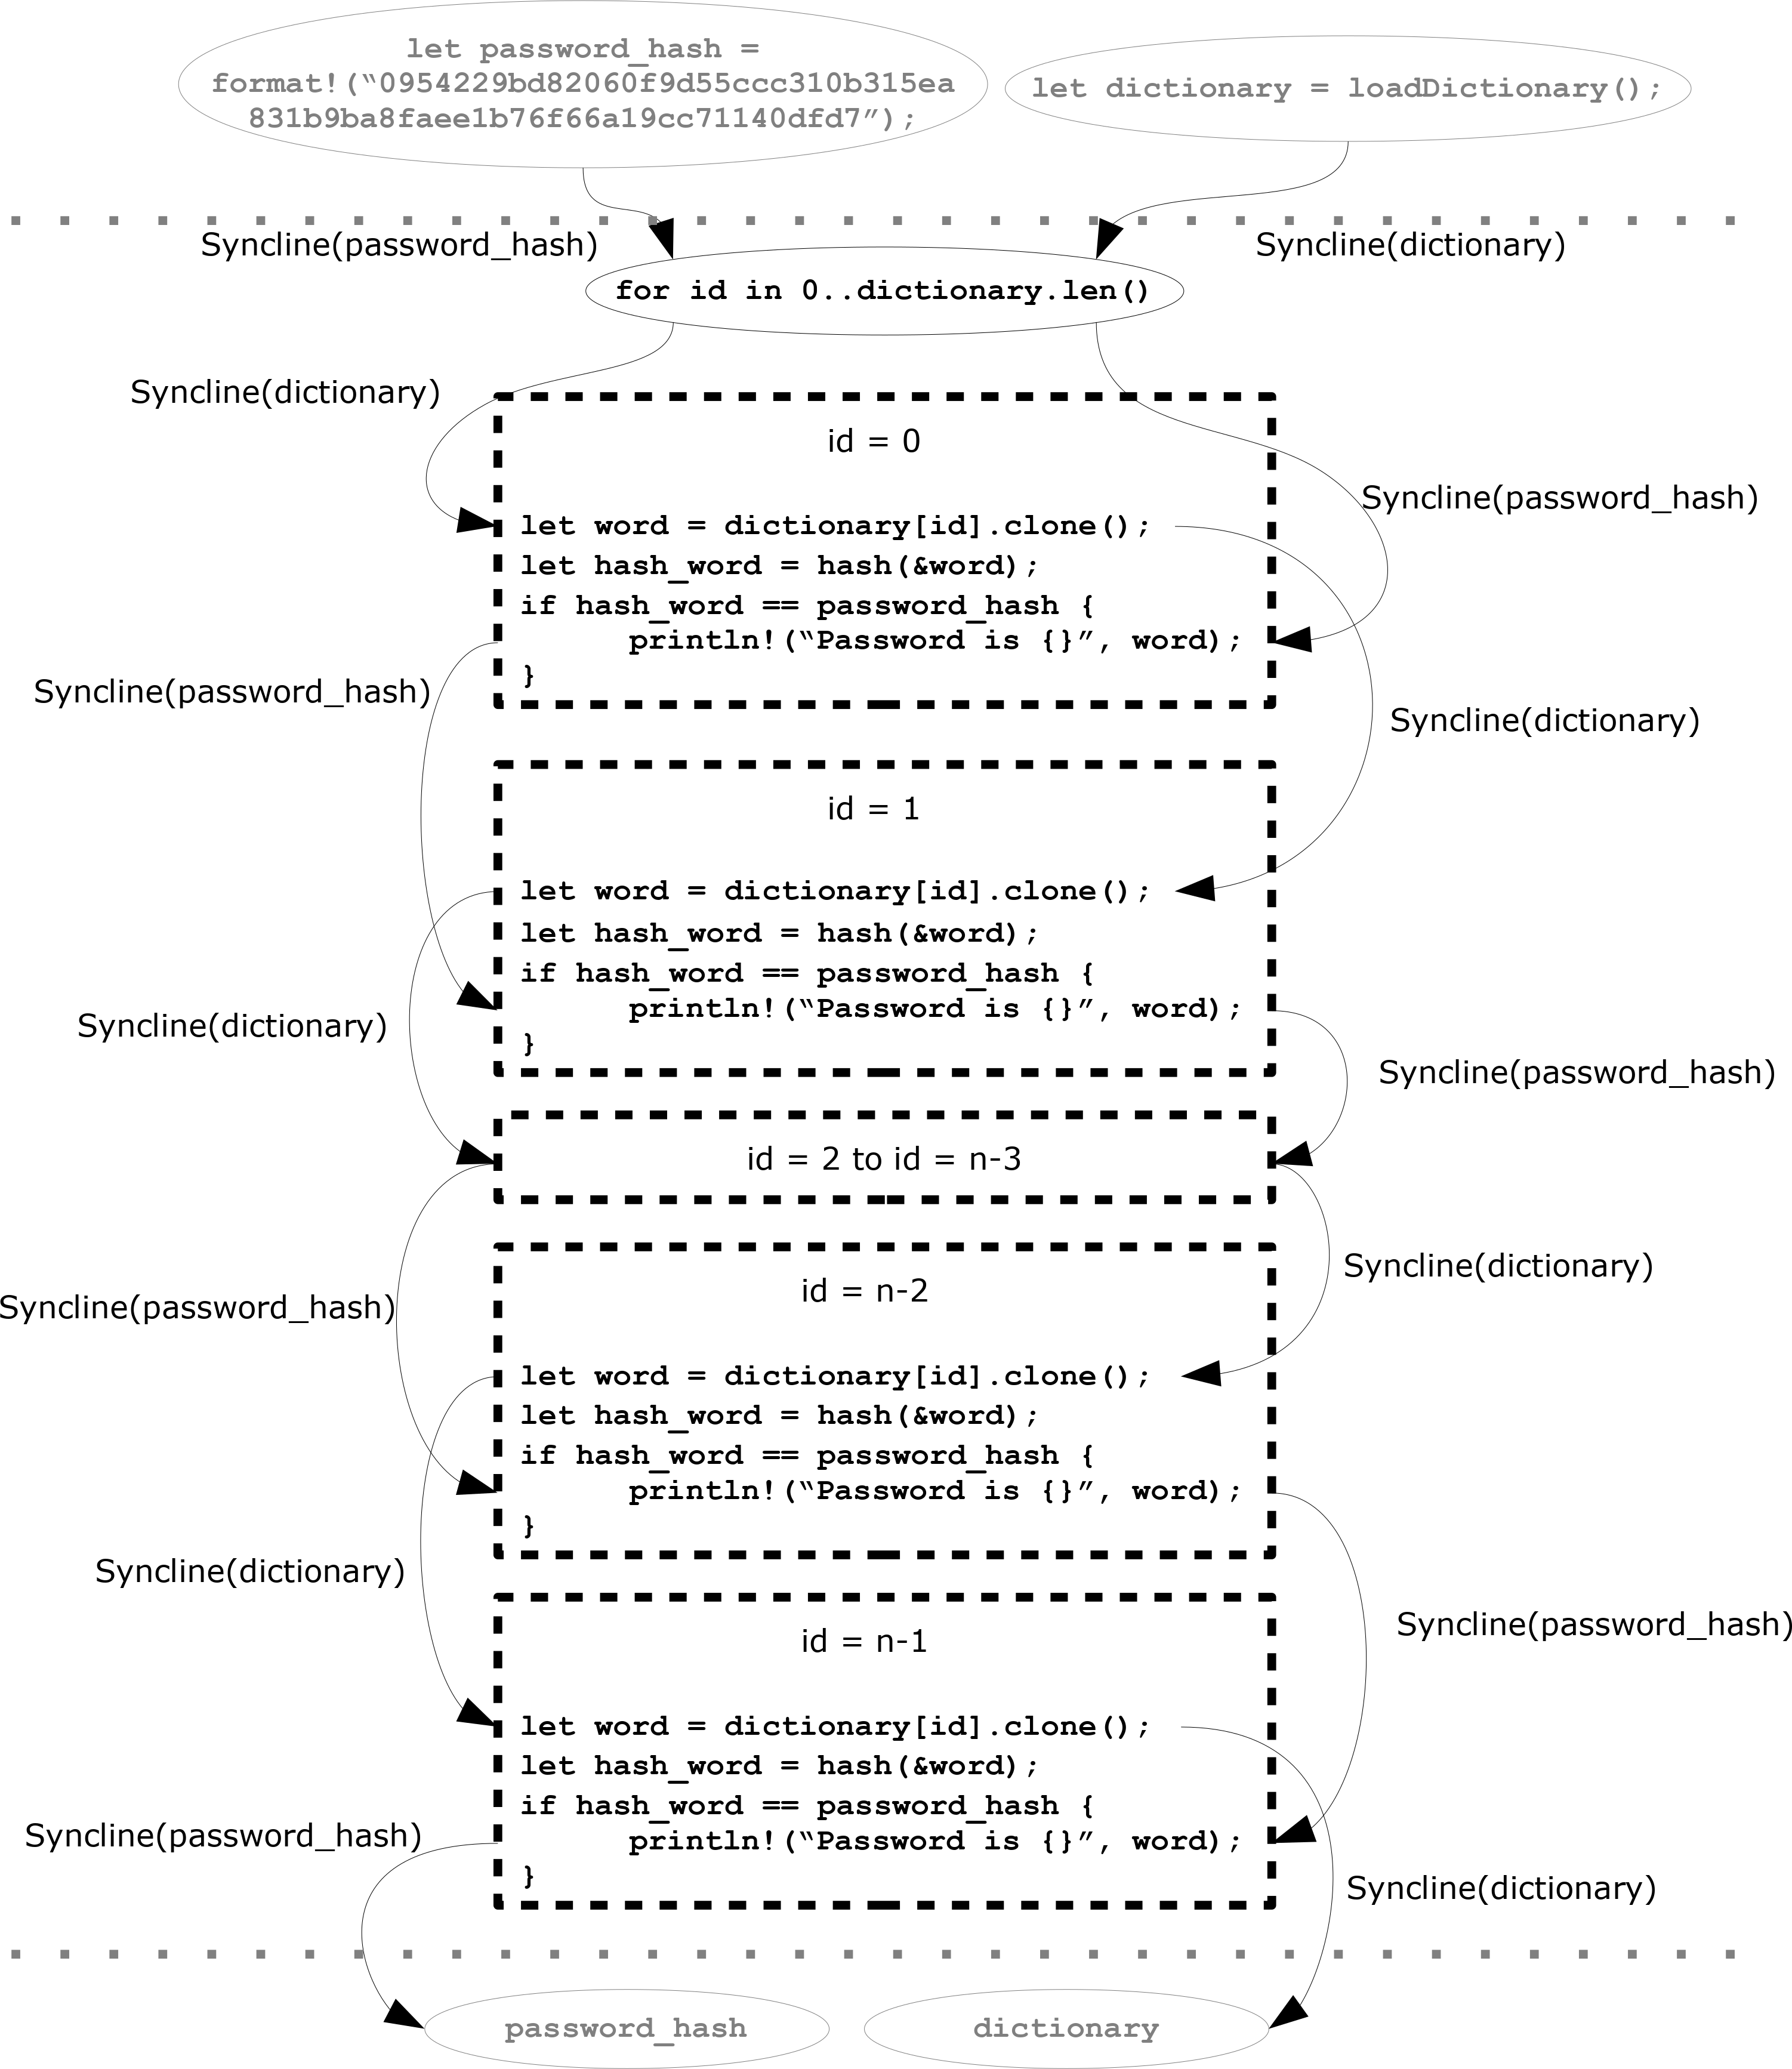
\includegraphics[width=\textwidth]{img/password-cracker/parallel-for.png}
    \caption{A schedule to show how the for loop in the main method from the password cracker program is parallelised}
\end{figure}

As you can see from this for loop schedule, the \texttt{dictionary} and \texttt{password\_hash} variables are requested on the first line they are required in the iteration and sent to the next iteration when they are no longer needed. In this case, only one statement uses each external dependency, so it is immediately released. The \texttt{hash} function is computationally expensive, and can only be started once it has access to its word in the dictionary. The dictionary can be passed very quickly through all of the threads, as accessing the element inside a list is very fast. This allows multiple \texttt{hash} functions to be run at the same time. The \texttt{password\_hash} variable is requested after the \texttt{hash} function returns, meaning \texttt{id=1} cannot check whether it is equal to the \texttt{password\_hash} if its \texttt{hash} function returns before \texttt{id=0}.

\subsection{Automatically Generated Sequential Programs}
To verify that the parallelising compiler can parallelise more that the programs shown above, it was tested against $100$ randomly generated sequential programs. Each randomly generated sequential program was executed sequentially and in parallel to compare the outputs. This is to verify that the program semantics remains the same. The sequential and parallel program was run $10$ times, and their execution time was recorded. The number of concurrent threads executed was also recorded for the parallel program. I am not expecting a speedup in the parallel programs as the size of the problem remained fairly small, and is probably not enough to overcome the thread overhead. The more interesting value will be the number of concurrent threads executed, as this shows how much parallelism the parallelising compiler could find in the sequential program. It gives us a gauge on how fast the parallel version could be if there was no thread overhead.

\todo{Show example of a randomly generated program?}

\section{Results}
\todo{Include results from automated testing}
